\documentclass{tufte-handout}
\usepackage{graphicx}

\title{Integers, Floats, and Arithmetic operators }

\author[The Academy]{Ilya Michurin}

%\date{28 March 2010} % without \date command, current date is supplied

%\geometry{showframe} % display margins for debugging page layout

\usepackage{graphicx} % allow embedded images
  \setkeys{Gin}{width=\linewidth,totalheight=\textheight,keepaspectratio}
  \graphicspath{{graphics/}} % set of paths to search for images
\usepackage{amsmath}  % extended mathematics
\usepackage{booktabs} % book-quality tables
\usepackage{units}    % non-stacked fractions and better unit spacing
\usepackage{multicol} % multiple column layout facilities
\usepackage{lipsum}   % filler text
\usepackage{fancyvrb} % extended verbatim environments
  \fvset{fontsize=\normalsize}% default font size for fancy-verbatim environments
  
  
  
    %MADNESS
  
  \usepackage[T1]{fontenc} % Use 8-bit encoding that has 256 glyphs
\usepackage{fourier} % Use the Adobe Utopia font for the document - comment this line to return to the LaTeX default
\usepackage[english]{babel} % English language/hyphenation
\usepackage{amsmath,amsfonts,amsthm} % Math packages
\usepackage{mathtools}% http://ctan.org/pkg/mathtools
\usepackage{etoolbox}% http://ctan.org/pkg/etoolbox
\usepackage{lipsum} % Used for inserting dummy 'Lorem ipsum' text into the template
\usepackage{units}% To use \nicefrac
\usepackage{cancel}% To use \cancel
%\usepackage{physymb}%To use r
\usepackage{sectsty} % Allows customizing section commands
\usepackage[dvipsnames]{xcolor}
\usepackage{pgf,tikz}%To draw 
\usepackage{pgfplots}%To draw 
\usetikzlibrary{shapes,arrows}%To draw 
\usetikzlibrary{patterns,fadings}
 \usetikzlibrary{decorations.pathreplacing}%To draw curly braces 
 \usetikzlibrary{snakes}%To draw 
 \usetikzlibrary{spy}%To do zoom-in
 \usepackage{setspace}%Set margins and such
 %\usepackage{3dplot}%To draw in 3D
\usepackage{framed}%To get shade behind text



\definecolor{shadecolor}{rgb}{0.9,0.9,0.9}%setting shade color
\allsectionsfont{\centering \normalfont\scshape} % Make all sections centered, the default font and small caps

% Standardize command font styles and environments
\newcommand{\doccmd}[1]{\texttt{\textbackslash#1}}% command name -- adds backslash automatically
\newcommand{\docopt}[1]{\ensuremath{\langle}\textrm{\textit{#1}}\ensuremath{\rangle}}% optional command argument
\newcommand{\docarg}[1]{\textrm{\textit{#1}}}% (required) command argument
\newcommand{\docenv}[1]{\textsf{#1}}% environment name
\newcommand{\docpkg}[1]{\texttt{#1}}% package name
\newcommand{\doccls}[1]{\texttt{#1}}% document class name
\newcommand{\docclsopt}[1]{\texttt{#1}}% document class option name
\newenvironment{docspec}{\begin{quote}\noindent}{\end{quote}}% command specification environment
\begin{document}

\maketitle % Print the title section

\begin{marginfigure}
  \includegraphics[width=\linewidth]{python-foundation-a-programmers-introduction-to-python-concepts-style-61-638.jpg}
  \label{fig:marginfig}
\end{marginfigure}


\normalsize



\section{Integers}
Python fully supports mixed arithmetic: when a binary arithmetic operator has operands of different numeric types, the operand with the ``narrower'' type is widened to that of the other, where plain integer is narrower than long integer is narrower than floating point is narrower than complex. Comparisons between numbers of mixed type use the same rule. The constructors int(), long(), float(), and complex() can be used to produce numbers of a specific type.


\normalsize

\marginnote[70pt]{\large{Numbers in brackets  Notes after this framed passage about arithmetic operators}}


\begin{framed}
\begin{verbatim}

x + y	sum of x and y	
x - y	difference of x and y	
x * y	product of x and y	
x / y	quotient of x and y	(1)
x // y	(floored) quotient of x and y	(5)
x % y	remainder of x / y	(4)
-x	x negated	
+x	x unchanged	
int(x)	x converted to integer	(2)
float(x)	x converted to floating point	
divmod(x, y)	the pair (x // y, x % y)	
pow(x, y)	x to the power y	
x ** y	x to the power y
\end{verbatim}
\end{framed}

\begin{marginfigure}
  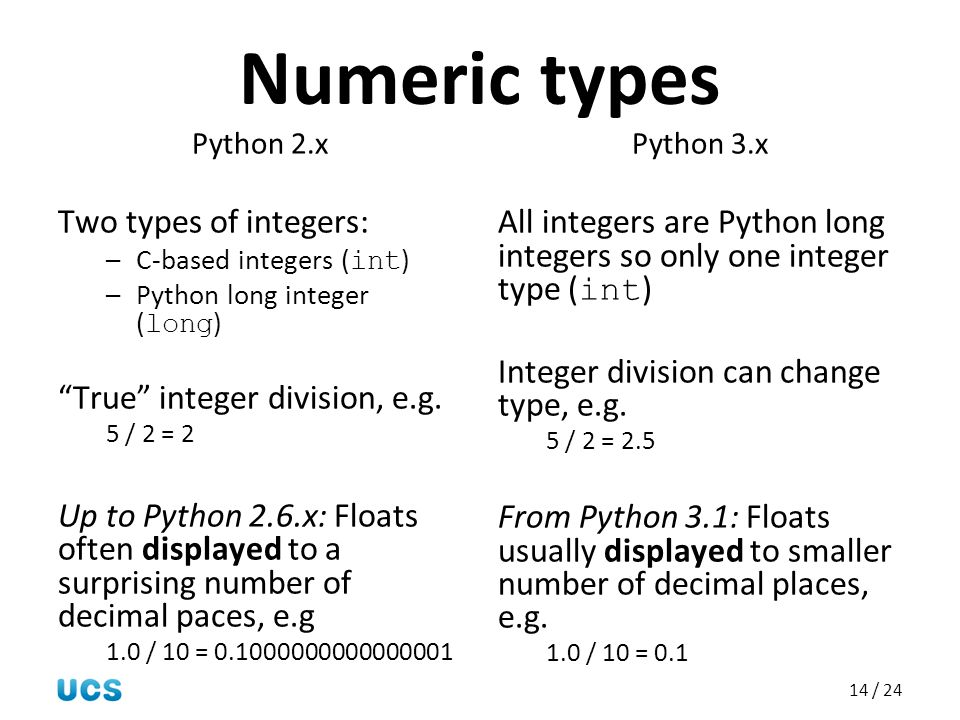
\includegraphics[width=\linewidth]{slide_14.jpg}
  \label{fig:marginfig}
\end{marginfigure}

\section{Notes}
For (plain or long) integer division, the result is an integer. The result is always rounded towards minus infinity: 1/2 is 0, (-1)/2 is -1, 1/(-2) is -1, and (-1)/(-2) is 0. Note that the result is a long integer if either operand is a long integer, regardless of the numeric value.

Conversion from floating point to (long or plain) integer may round or truncate as in C; see functions floor() and ceil() in the math module for well-defined conversions.

Complex floor division operator, modulo operator, and divmod().
Deprecated since release 2.3. Instead convert to float using abs() if appropriate.

Also referred to as integer division. The resultant value is a whole integer, though the result's type is not necessarily int.

\bibliography{sample-handout}
\bibliographystyle{plainnat}


\begin{shaded}
\begin{verbatim}

As the result, we got 

continuous creation of "New States" which you can stop
only by killing the program 

Because we couldn't put changing of live cells 
in one state

\end{verbatim}
\end{shaded}
















